I missed the two morning talks, sadly!

\subsection{Fiery Cushman on How We Know What Not to Think}
\label{sec:fc}

The lab studies two things: 1) Decision-making, and 2) Morality. \\

$\ra$ Often trying to find two ways to study {\it both} subjects simultaneously (how can we gain insights across these two fields?). \\

{\bf Decision-Making:} Roughly two kinds; planning vs. habit (system 1 and system 2, and so on). Sometimes seen as competitors. \\

Q: Can these two processes be integrated? \\

A: Yes! Today, let's discuss how habitual decisions can be used to make planning and model-based reasoning more intractable. \\

{\bf Game:} 20 seconds to answer a question:
\begin{itemize}
    \item Q: If you could have anything you want for dinner tonight what would it be?
    
    (my answer: Andina in Portland, Oregon!)
    
    $\ra$ One MTurker emailed them and said: ``I don't need 20 seconds to determine I want lasagna"
    
    \item Q: How many people considered one thing? (some hands)
    \item Q: How many people considered multiple things? (more hands)
    \item Some experiments: do you want a hot dog or grilled cheese?
    
    $\ra$ Easier to choose in this case!
\end{itemize}


{\bf Problem:} without constraints on the space (grilled cheese/hot dogs), how do we decide which food to think about? There are {\it so many conceivable things} (to eat). \\

\dbox{{\bf Guiding Question:} How do we determine which things to consider among these massive spaces of conceivable things? \\

$\ra$ Answer tl;dr: We use one system to generate the space of conceived things, and another system to choose among them}

That is:
\begin{enumerate}
    \item {\bf Model-free:} We use cached/model-free reasoning to generate cached thins
    \item {\bf Model-based:} Search and choose among this space.
\end{enumerate}

\subsubsection{Experimental Methodology for Understanding Conceivability Space}

Experimental setup:
\begin{itemize}
    \item Ask MTurkers: if you could have anything you want for dinner, what would it be?
    \item Answer: $__________$, could be any number of things! (not just one, necessarily)
    \item Track the answers and the {\it number} of answers.
    
    $\ra$ Also interested in the relationship between time givent to answer and number of answers.
    
    \item Then ask: compared to all the things you eat, how much do you like this? How often to do you eat this?
\end{itemize}

Hypothesis: cached value of items contributes to choosing among a conceivability set. \\

$\ra$ Finding: the foods that come to mind are the ones people {\it value} not the ones you eat {\it often}. See Figure~\ref{fig:food}.


\begin{figure}[h!]
    \centering
    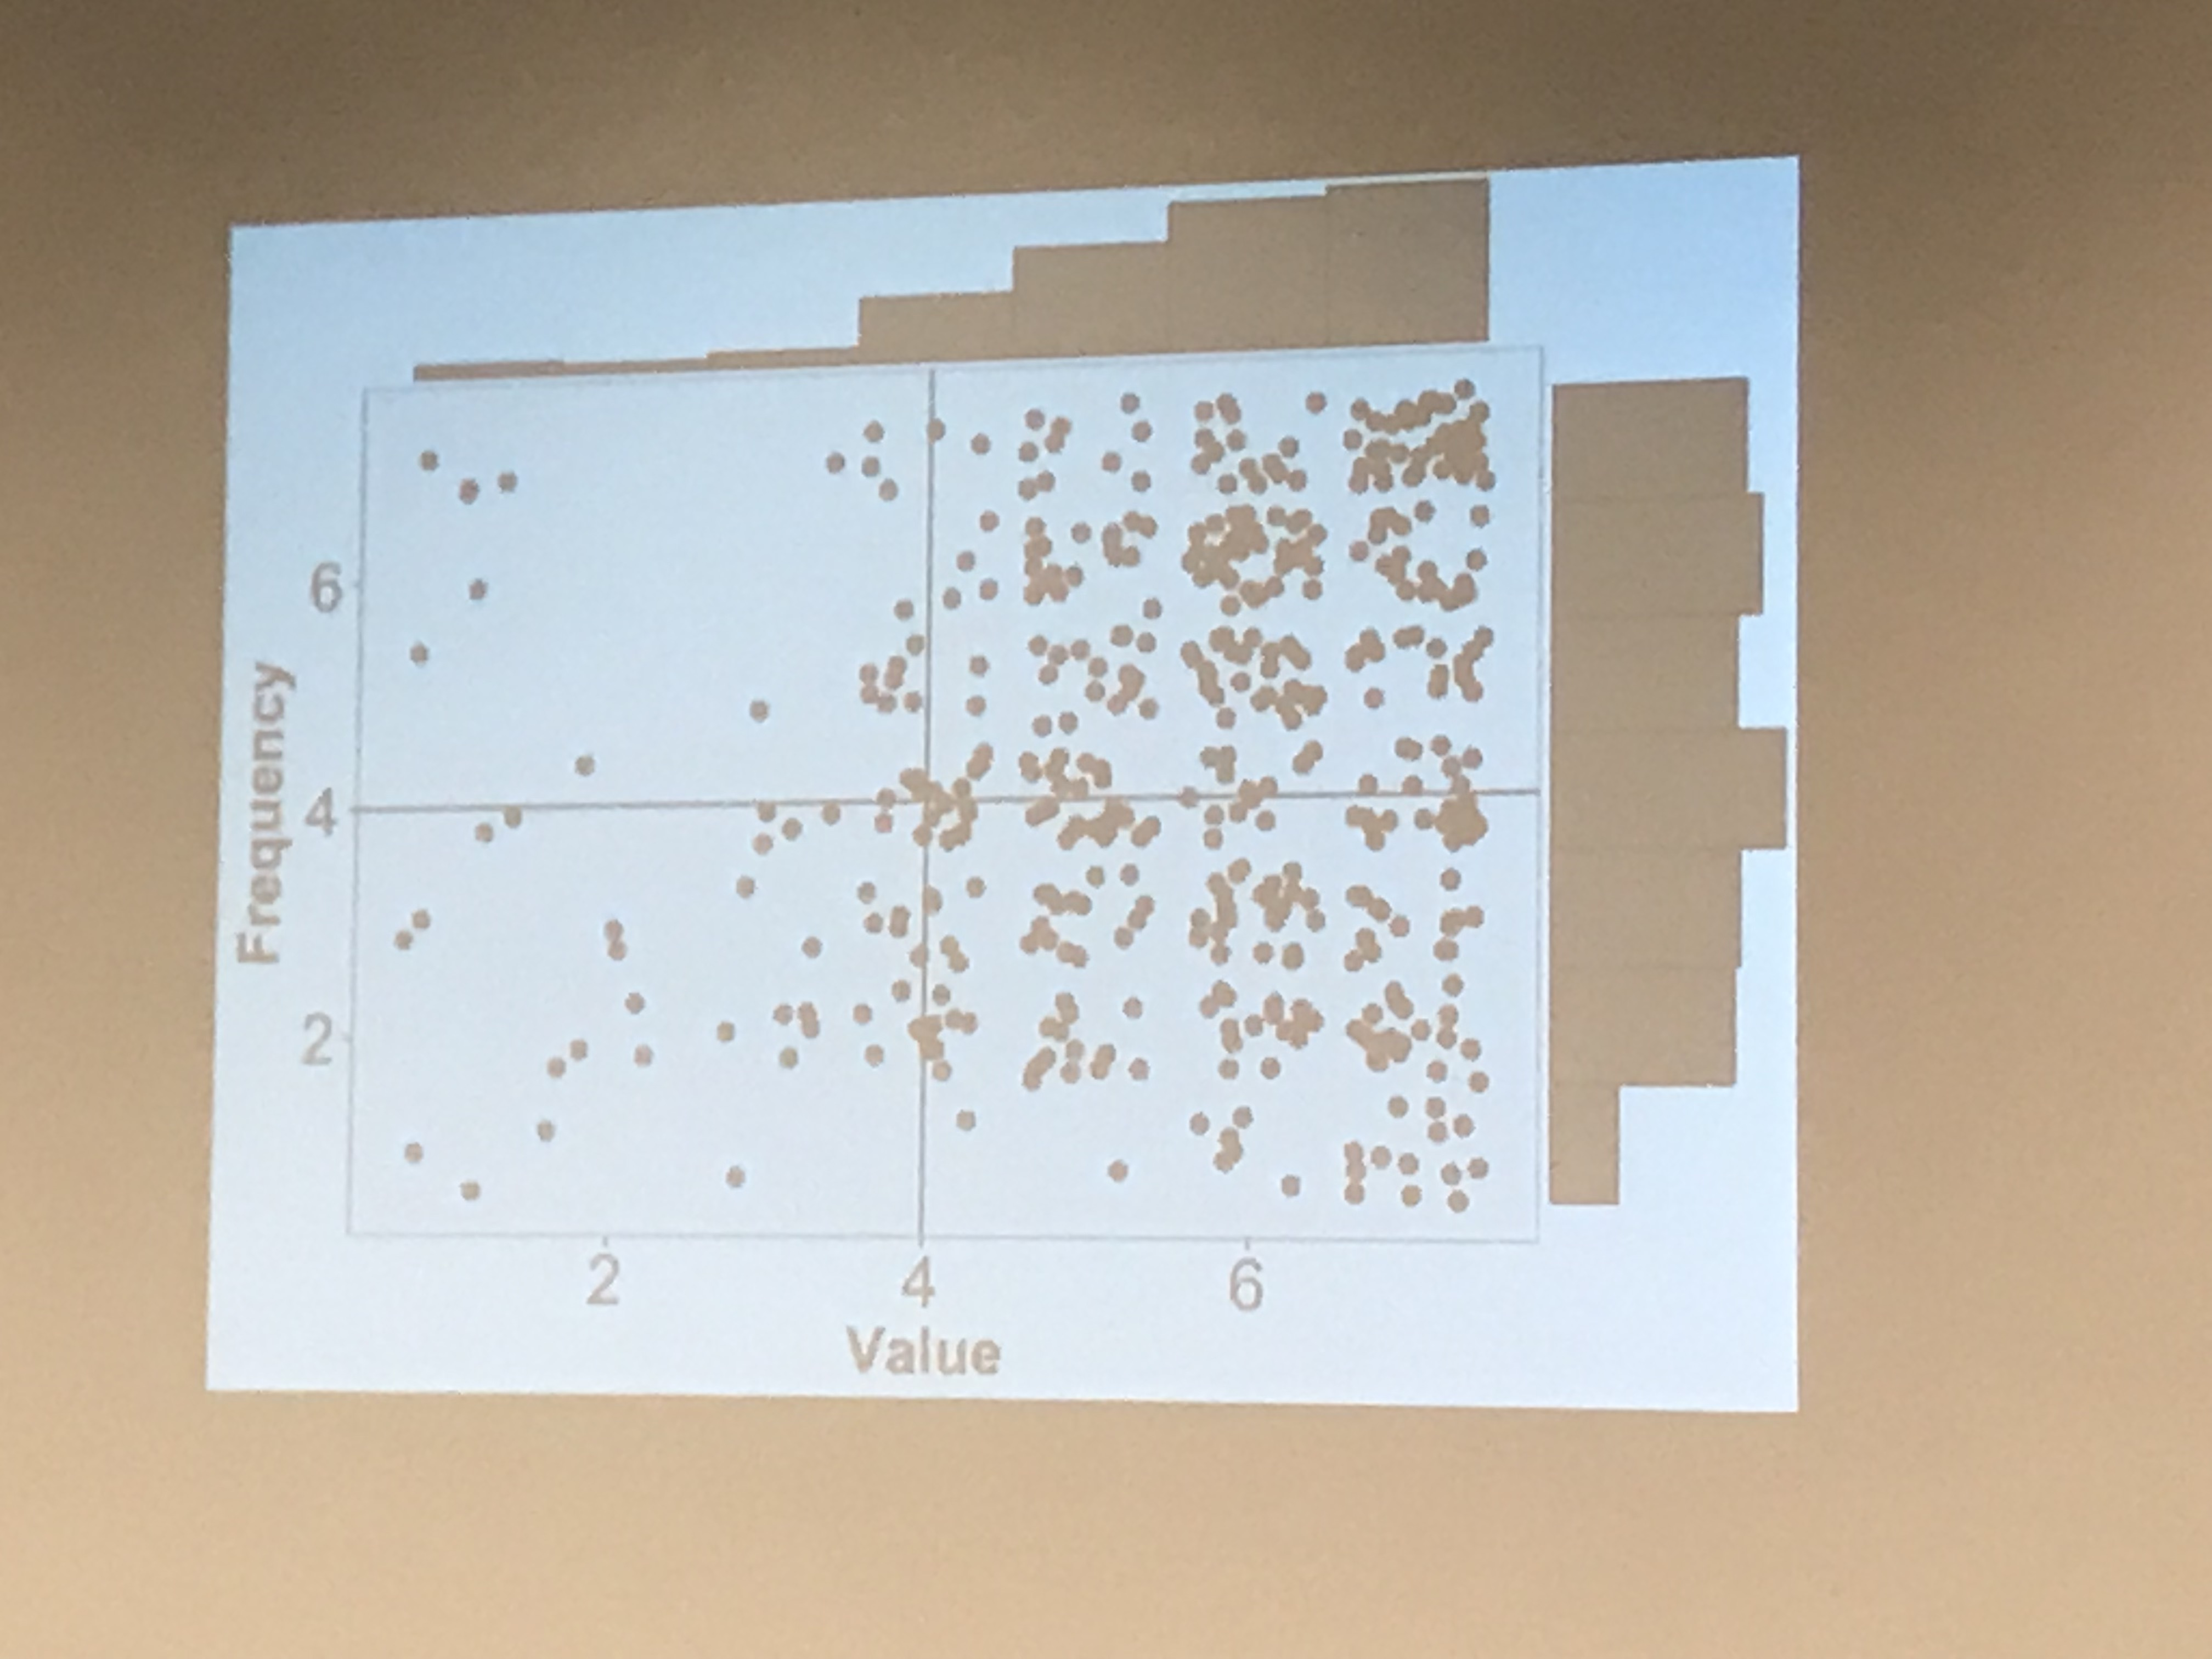
\includegraphics[width=0.5\textwidth]{images/food.JPG}
    \caption{Value vs. Frequency of foods considered.}
    \label{fig:food}
\end{figure}


\subsubsection{Two Systems Used for Conceiving}

Example: you are cooking dinner for a friend who broke his leg. You won't eat this dinner. You have \$40 and 45min to cook. Your friend is allergic to seeds doesn't like food to moist and hates chewy food. What do you cook?

$\ra$ Can test this hypothesis: what do you like in general? Vs. what do you consider for your friend, today? \\

{\bf Model:} based on a contextual bandit~\cite{li2010contextual}. See Figure~\ref{fig:cb}.

\begin{figure}[h!]
    \centering
    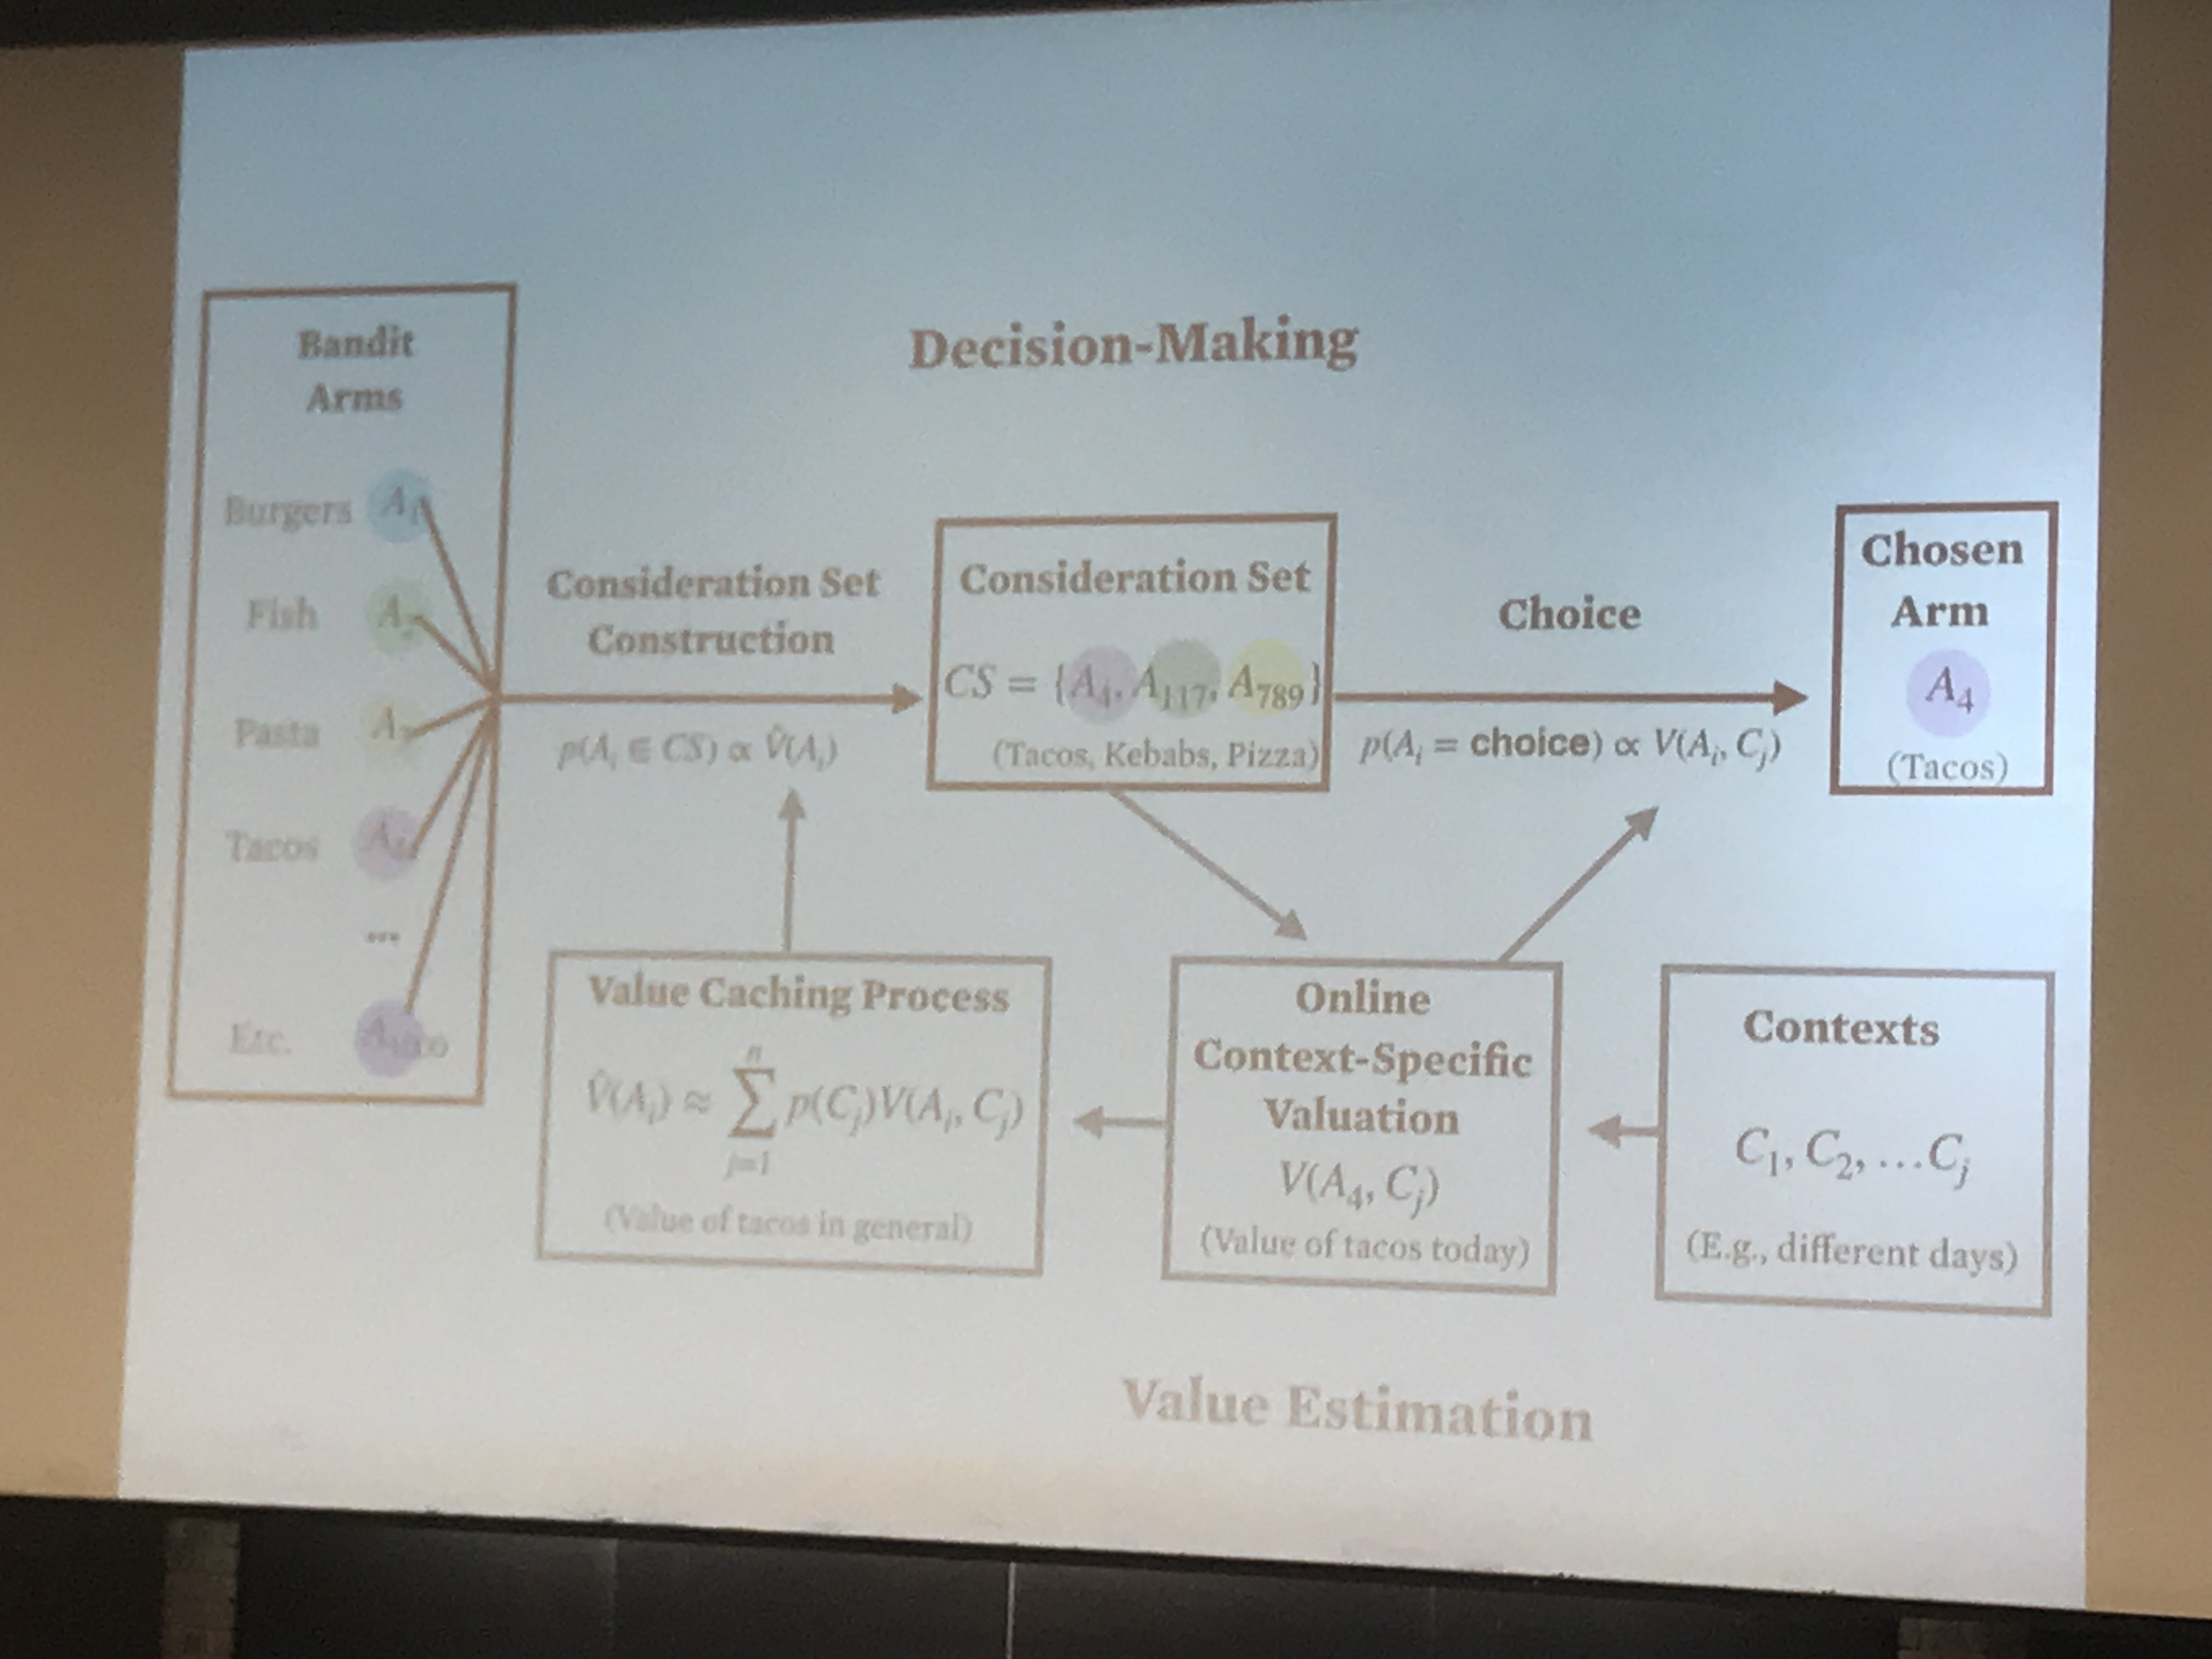
\includegraphics[width=0.5\textwidth]{images/cb.JPG}
    \caption{Contextual bandit for modeling this decision making process.}
    \label{fig:cb}
\end{figure}

Experiment:
\begin{itemize}
    \item Compare fraction of cognitive effort (relative to exhaustive online evaluation) vs. Fraction of average payoff obtained.
    \item Makes a big difference: correlation between cached context vs. no context.
    
    $\ra$ Explore whether basing the choice set on the current context has an impact on decision making.
    
    \item Q: What does pure model-free decision making look like? Well, it's greedy with respect to value estimates.
    
    $\ra$ But, again, we might expect that the context determines a choice set, then the model-based decision making kicks in.
    
    \item {\bf Finding:} More cognitive effort leads to more payoff, but at diminishing returns.
\end{itemize}

Experiment:
\begin{itemize}
    \item Give MTurkers the above prompt (cooking for a friend).
    \item Then, ask the same questions from before: how much do you like this food? How often do you eat it? And so on.
    \item {\bf Finding:} no effect of situational value on decision, but high impact of general value.
\end{itemize}

Follow Up Experiment:
\begin{itemize}
    \item Also run the ``month-of-the-year" study: associate \$ to each month, subjects strongly associate value with different months. Then, give them a new value, and tell the subjects 
    
    Ex: word problem, only answers are months of the year. ``For which month is its 3rd letter closest to z".
    
    $\ra$ 40\% think of Nov, 40\% think of May (right answer!).
    
    \item Main question: how much does the value from the {\it previous} study (assigning value to months) determine which months people think of?
    
    $\ra$ {\bf Finding:} Correlation between which months were valued in the study and how often they are considered (either along the way).
\end{itemize}


Next Experiment:
\begin{itemize}
    \item New prompt: what food do you {\it least} want to eat? (Or, similarly: what's the worst month?)
    
    $\ra$ Contrast this with people asked what's the best food/month?
    
    \item {\bf Finding:} when people are asked to think of bad foods, {\it they still tend to think of good foods}.
    
    $\ra$ Not the case when asked about good food; that is, people don't think of bad foods along the way.
\end{itemize}

**Not suggesting the only way we construct consideration sets is through value sets. Other ways, too: contextual memory/semantic memory (call up a list of crunchy foods), and so on. \\

More on this work in paper by~\citet{morris2018causal}.


\subsubsection{What is ``Possible"?}

Example: where should you take your friend to eat? Oh and by the way the friend is vegetarian. You say: ``let's get burgers!" Philosopher says: ``Yes, that's {\it possible}" (conceivable, etc.). \\

Practical notion of possible:
\ddef{Possibility}{Possibility, in this context, is better thought of in terms of feasibility/realism; do what extent is this achievable, practically?}

To contrast to philosophers' definition where we really mean something like logical/metaphysical possibility. \\

Experiment: 
\begin{itemize}
    \item Adam is driving to airport and his car breaks down. We'll be asked under different time pressures (1sec vs 15sec).
    
    \item We got the 1sec condition: ride a cat to airport, ride a taxi without paying, run to the airport, call a friend, and so on.
    
    \item Examine effect of time given to answer on whether people think things are possible. That is, given 1sec vs 15sec, which things did people find were possible/impossible?
    
    \item {\bf Finding:} For impractical actions there was little difference between the fast (1sec) and slow (15sec) decision groups.
    
    $\ra$ {\it Huge effect:} for {\it moral} decisions, massive difference between fast/slow.
    
    $\ra$ Ex: ask a four year old: can you grow bananas with lightning? The child answers: No! Is it possible to steal a candy bar? The child answers: No!

    $\ra$ For more on morality in decision making, see work by~\citet{baron1997protected,crockett2017moral}.
\end{itemize}

\subsubsection{Why is Morality Different in Conceivability?}

Q: Why is morality so different from the other cases? 

A: Imagine you're in a grocery store and think about stealing a candy bar. If we arrange these outcomes according to value, we'd see that the majority of outcomes have negative outcomes. \\

$\ra$ Let's think about this as a contextual bandit: what is the value of each of these actions? \\

Experiment:
\begin{itemize}
    \item Only two outcomes: you get caught or you don't get caught, changes based on context (as in a contextual bandit).
    \item Also have access to a context free value assessment. So, two decision strategies (context free vs. context based):
    \begin{align}
        &\max_a V(a, C_j)\hspace{10mm} \max_a \hat{V}(a) \approx \nsum p(C_i) V(a,C_i).
    \end{align}
    
    \item Given different amount of data, should use different strategies.
\end{itemize}

{\bf Proposal:} Because morality involves decisions that often include {\it catastrophically bad} but unlikely outcomes, model-free decision making seems particularly poignant in excluding immoral options in the first place. \\

Final Experiment:
\begin{itemize}
    \item Q: do ordinary people understand that morality constrains the thoughts that come to mind?
    \item Setup: describe an escape room (the social game) to a group of people.
    $\ra$ Then: someone will ask, how should we get out? 
    
    $\ra$ Prompt: ``Bill thought for a moment, the first thing that came to mind was that they could cut his teammate Frank's arm off, but he thought would be obviously wrong and so he kept thinking of other possibilities and didn't answer Kat's question until he thought of a better one'
    
    \item Moral psychology says this is the {\it right thing} because he has the same morals as us.
    
    \item But! People responded to the prompt: ``that is a horrible thought, it's terrifying that the first thought was this" and so on.
    
\end{itemize}

Concluding Remark:
\begin{enumerate}
    \item People are not able to think without being constrained by social norms.

    \item The kinds of planning problems we routinely engage in are made efficient by these constraints and other norms.

    \item These norms structure our thought processes by handing to us the right options on a silver platter, by excluding useless or wrong thoughts.
\end{enumerate}

\spacerule

\subsection{Amy Zhang On Learning Causal States of Partially Observable Environments}

Joint work with Joelle Pineau; Laurent Itti; Zachary Lipton; Tommaso Furlanello; Kamyar Azizzadenesheli; and Animashree Anandkumar. \\

Alternate view of RL: Predictive State Representations (PSR)~\cite{littman2002predictive}. \\

\ddef{Predictive State Representations}{PSRS are vectors of predictions for a specially selected set of action-observation sequences, called tests.}

$\ra$ Nice property of PSRs: by definition sufficient statistic for future action-observation sequences. \\

Core test: linearly independent columns of $D$
\[
Q = \{q_1, \ldots, q_k\}.
\]
$p(Q \mid h)$ is a sufficient statistic of $h$ for $p(t \mid h)$. \\

But! Doesn't scale. \\

\dbox{{\bf Core Contribution:} Learning PSRs with gradient-based methods.}

$\ra$ Use ideas from causal models!

\ddef{Causal Model}{A causal model has the ability to understand how to manipulate the world, robust to changes in behavior.}

Q: What is the notion of causality that is useful and learnable in RL? \\

A: Expanding on PSRs: causal states. \\

$\ra$ Consider a stochastic process $y_{t-1}, y_t, \ldots$. \\

$\ra$ Causal equivalence relation $\sim_\eps$:
\[
y \sim_\eps y' \equiv \Pr(Y \mid Y = y) = \Pr(Y \mid Y = y').
\]
\ddef{Causal States~\cite{crutchfield1989inferring}}{The causal states of a stochastic process are partitions $\sigma \in \mathbb{S}$ of the space of feasible pasts $Y$ induced by the causal equivalence.}

Method: minimal sufficient statistics can be computed from any other non-minimal sufficient statistic. \\

$\ra$ Components: recurrent encoder, next step prediction network, discretizer, a second prediction network. \\

Two Learning Objectives: 1) sufficiency, and 2) knowledge distillation:
\begin{align}
    &\min_w \sum_t^T L_T\left(\Pr(O_{t+1} \mid o, a, a_t), \Psi(o, a, a_t)\right). \\
    &\min_w \sum_t^T L_T\left(\Psi(o, a, a_t), \Lambda(o,a,a_t)\right).
\end{align}

{\bf Experiments:}
\begin{itemize}
    \item {\it Stochastic System}: explore whether the system can handle stochastic dynamics, high dimensional stochastic observations.
    
    $\ra$ Domain with integer ground truth states with stochastic dynamics
    
    $\ra$ Using just the observation yields poor performance (expected), while the PSRs help.
    
    \item Next up are some partially observable gridworlds. Pick up key to unlock a door then move to goal.
    
    $\ra$ As environments get more complex
    
    \item {\it 3D Maze:} Reward can be in two different arms of a T maze, receive first-person observations.
    
    $\ra$ Agent has to learn a representation that incorporates the information about which task it's in.
    
    $\ra$ With causal states, can consistently find the goal.
    
    \item {\it Atari Pong:} only see a single frame, so it's partially observable.
    
    $\ra$ Causal state representation is able to determine relevant information from observations and perform well.
\end{itemize}

Two contributions:
\begin{enumerate}
    \item A gradient base learning method for PSRs.
    \item A notion of causality and discretization to achieve causal states.
    $\ra$ Causal states give additional interpretability.
\end{enumerate}


\spacerule

\subsection{Rich Sutton on Play}

Eight years ago we started this thing! And I thought some day maybe I'll be able to speak the group: really happy to be here because I've never gotten to speak to this group. \\

$\ra$ This is a great meeting. So many diverse people thinking about how the mind works: goals, rewards, cognition. A clear focus! I hope we can keep doing it. \\

Here: how I've been thinking about this awesome problem of understanding the mind. \\

\subsubsection{Integrated Science of Mind}

{\bf Point:} There should be an {\it integrated science of mind} (ISM) that applies equally well to people, animals, and machines.
\begin{itemize}
    \item Because all minds have essential commonalities
    \item Because in the foreseabble future many minds will be machine minds
    \item Because an ISM does not rest easily whtin any existing field: psych? AI? Cog Sci?
    \item Maybe the RLDM community is the beginning of such an Integrated Science of Mind?
\end{itemize}

``Intelligence is the computational part of the ability to achieve goals' (John McCarthy), with Rich saying ``Mind" is the appropriate term instead of ``intelligence". \\

Let's talk about play! Goals are key. And goals are key to what mind is. \\

\ddef{The reward or RL hypothesis}{Goals and purposes can be well thought of as maximizing the expected value of the cumulative sum of a single received signal (called reward)}

Rich attributes the above to Michael, Michael attributes it to Rich (and that's their deal!) \\

Two key points:
\begin{enumerate}
    \item Reward is a singular goal, so any subgoal must be subservient to it
    \item Reward cannot change.
\end{enumerate}

These two things will come back at us. Especially in regard to Play. \\

The RL landscape right now:
\begin{itemize}
    \item {\bf Goals:} In core RL we learn Value Functions and policies (these are where goals fit well).
    
    $\ra$ We have sort of done this!
    
    \item {\bf Subgoals:} Next, we need to learn: states, skills, and models.
    
    $\ra$ We need to do this more/next!
    $\ra$ Not necessarily directly about reward
    $\ra$ Q: How should the learning of these things be structured to make a coherent mind? We have to get reward because it's the meaning of life.
\end{itemize}

**Play is massively important to this second category.


\subsubsection{What Is Play?}

Some nice videos of animals playing with different items: an orca whale nudging a floating barrel, an orangutan learning how to swing on a branch, a snake pushing a ball around, and a cat playing with a toy. \\

$\ra$ Babies are famous for playing as well (shows some videos of some babies playing). \\

$\ra$ It's all purposeful but purposeless at the same time. How can that be? \\

Play Quotes:
\begin{itemize}
    \item ``Play is a critically important activity that is basic to human nature, society, culture, and history, and has an essential role in learning and human development"---National Museum of Play
    
    \item ``True object of all human life is play"---G.K. Chesteron
    \item ``Play is hard to maintain as you get older. You get less playful. You shouldn't of course."---Feynman
    
    \item ``play is a free activity standing quite consciously outside ordinary life as being not serious but at the same time absorbing the player intensely and utterly"---Johan Huizinga
    
    \item ``Competition can turn play into non-play if rewards for winning extend beyond the game itself"---Peter Gray
\end{itemize}

$\ra$ Almost by definition it has to be useless! \\

Rich's take on play ``Play is the pursuit of subgoals seemingly unrelated to the main goal (reward) but which may end up helping the main goal in some way in the long term."
\begin{enumerate}
    \item Play is like research! Some thing are pursued because they are interesting
    \item Some things are pursued because they are sometimes valued.
\end{enumerate}

\subsubsection{Subproblems}

Long history in AI/RL looking at subproblems that are nominally distinct from the main problem:
\begin{itemize}
    \item Curiosity in RL (Schmidhuber 1991, Others)
    \item Multiple learning asks improve generalization (Caruana 1993-1997, Baxter 1997)
    \item Large numbers of off policy RL tasks as learning a model (Sutton 1995, 1999, 2011)
    \item Skills/Options (Many 1999---)
    \item Instrinic Motivation in RL
    \item Auxiliary RL tasks improve generalization (Jaderberg 2014)
    \item Here: Oudeyer, Harutyunyun, Xia, Foster, Mattar, Mcilrath, Dabney, Hoffman.
\end{itemize}

Q: Are subtasks distinct from subgoals distinct from subproblem? \\

A: Most neutral term is {\it subproblem}. Some problem that is subsidiary to the main problem. \\
Q: What do we agree on regarding subproblems? \\

A: Well, at least two things:
\begin{itemize}
    \item Subproblems are a reward and possibly a ``terminal" value (subgoals).
    \item The solution to a subproblem is an option---a policy and a way of terminating.
\end{itemize}

Perhaps there are really two things going to here that {\it we need}:
\begin{enumerate}
    \item The pursuit of particular arbitrary subproblems.
    \item The pursuit of learning progress (exploration).
\end{enumerate}

\subsubsection{Some Answers to Three Open Questions About Subproblems}

Three key questions about subproblems:
\begin{enumerate}
    \item {\it What should the subproblems be?}
    
    $\ra$ Rich A: Each subproblem should seek to turn a state feature on while respecting the original rewards.
    
    $\ra$ Formally: the subproblem for feature $i$ has same rewards plus, if the option stops at tine $t$, then when transitioning to $s_t$, receive
    \[
    V(s_t) + \tx{bonus}_i \cdot x_t^i.
    \]
    Where ``bonus" is set proportional to variability in the weight for feature $i$.
    
    \item {\it Where do they come from?}
    
    $\ra$ Rich A: Subproblems come from state features! There is one subproblem for each feature whose contribution to the value function is highly variable.
    
    
    \item {\it How do they help the main problem?}
    
    $\ra$ Rich A: The solution to a subproblem is an option that turns its feature on; With this, one can act decisively to achieve the feature, and plan in large abstract steps of feature achievement as the value of features change.
\end{enumerate}



{\bf Q: First, how do the subproblems help the main problems?} \\

A: A few ways!

\begin{enumerate}
    \item By shaping the {\it state representation}
    
    $\ra$ Feature reps that are good for subproblem may also be good for the main problem.
    
    \item By shaping {\it behavior}.
    
    $\ra$ Learn a good set of options.
    
    \item By enabling {\it planning at a higher level}.
    
    $\ra$ Subproblems$\implies$Options$\implies$transition models which can be used in planning.
    
    $\ra$ Planning helps when states change values.
\end{enumerate}

Example: Now let's take some time to think about sitting down to eat a meal. You have to pick up utensil to eat, maybe put the fork down, pick up the spoon, and so on. {\it You have goals and values are changing all over the place.} You could say nothing changes; earlier I put food in mouth, now I want water. Or, you could say your moment by moment values change. \\

$\ra$ Let's explore this idea a little bit. It's a decent way to think: I need to do this mechanical activity. A huge planned activity. A goal-directed thing learned based on subgoals. \\

{\bf Proposal:} we should have bonuses for achieving features. Most common in literature: a new reward function. But let's keep the old reward function! I still don't want to stab myself when I pick up the fork. When I put down the water glass, I still don't want to spill everywhere. \\

$\ra$ Feasible then to generate subproblems. \\

{\bf Q: Second, where do the subproblems come from?} \\

Another Q: Well, first why might the values of state features change? \\

Answers: 1) Because world hanges, 2) Because our policy changes as we learn, and 3) Because the world is big, and we encounter different parts at different times. \\

$\ra$ We should embrace the idea that {\it the world is much more complex than the mind.} The mind is too small to contain the exact value function! There will not be enough weights. Therefore:
\begin{itemize}
    \item We must embrace approximation
    \item The best approximate value function will change {\it even if the world does not.}
    
    $\ra$ A big world $\implies$ non-stationary
\end{itemize}

Permanent and transient memories in value function approximation~\cite{sutton2007role}. \\

Example: consider Go. A black stone in the middle of a 5$\times$5 square is good. Others might be too, but this is the best. But, in other positions, can learn exceptions from long term ``good" features. For more see work by~\citet{sutton2007role}. \\

Two thoughts to conclude:
\begin{itemize}
    \item Remember our RL landscape (see first section of talk).
    \item But, now: instead of states, we'll talk about state features; instead of skills, we mean options, instead of models, we mean models of options.
\end{itemize}

Summary:
\begin{itemize}
    \item RL is entering a new phase attempting to learn much more ambitious things: states, skills, and models, all having to do with subgoals.
    
    \item Play highlights the need for this ambition and highlights the importance of subproblems in mental development
    
    \item State-feature subgoals, respecting reward, are a distinctive form of subproblem.
    
    \item The world is big! We must approximate it, which yields non-stationarity. Provides a rationale for play and planning.
    
    \item Problems of subproblem selection and of exploration/curiosity may be separable; both are needed before our agents will play.
\end{itemize}


Audience Question: How should we be thinking of states?\\

Rich: A state is a summary of past experience that's good for predicting the future. So, is it a good input to your value function/policy/model? What is our ideal state, then? I want to define everything in terms of experience and data and not in terms of human theories about the world. So, based on data, not theories. Whatever we mean about the world has to be translatable into statistical statements about our data stream of experience. What does it mean to be a podium.

\spacerule

